\documentclass[11pt, a4paper, twocolumn]{article}

% ---------- Packages ----------
\usepackage[utf8]{inputenc}
\usepackage[T1]{fontenc}
\usepackage{mathptmx}                  % Times New Roman
\usepackage[left=1.5cm, right=1.5cm, top=2cm, bottom=2cm]{geometry}
\usepackage{setspace}
\singlespacing                          % Single spacing
\usepackage{graphicx}
\usepackage{booktabs}
\usepackage{natbib}
\setcitestyle{round, aysep={}}          % Harvard-style: (Author Year)
\bibliographystyle{plainnat}            % Author-year Harvard style per B&E: PRIA
\usepackage{hyperref}
\usepackage{xcolor}
\definecolor{navyblue}{RGB}{0, 0, 128}
\hypersetup{colorlinks=true, linkcolor=navyblue, citecolor=navyblue, urlcolor=navyblue}
% \usepackage{lineno}                   % Line numbering (disabled for final)
\usepackage{caption}
\captionsetup{font=small, singlelinecheck=false}
\usepackage{amsmath}
\usepackage{float}                      % [H] placement for figures

% ---------- Section formatting: numbered, normal case ----------
\usepackage{titlesec}
\titleformat{\section}{\normalfont\large\bfseries}{\thesection.}{0.5em}{}
\titleformat{\subsection}{\normalfont\normalsize\bfseries}{\thesubsection.}{0.5em}{}
\setcounter{secnumdepth}{2}             % Number sections and subsections

% ---------- Running headers ----------
\usepackage{fancyhdr}
\setlength{\headheight}{14pt}
\pagestyle{fancy}
\fancyhf{}
\fancyhead[L]{\small\textsc{Biology and Environment}}
\fancyhead[R]{\small\textsc{Predicting the distribution of} \small\textit{S.~nobilis}}
\fancyfoot[C]{\thepage}
\renewcommand{\headrulewidth}{0pt}

% ---------- Figure caption format: Fig. N--- ----------
\DeclareCaptionLabelFormat{beformat}{Fig.~#2}
\DeclareCaptionLabelSeparator{emdash}{\textemdash}
\captionsetup[figure]{labelformat=beformat, labelsep=emdash, font=small, singlelinecheck=false}

% ---------- Document ----------
\begin{document}

\twocolumn[{%
\centering
\vspace{1em}
{\large\bfseries\MakeUppercase{Predicting the expanding distribution of \textit{Steatoda nobilis} in Western Europe using satellite observations of artificial light and land surface temperature}\par}
\vspace{1em}
{Eoin P. Carley and Ruth A. Power\par}
\vspace{0.5em}
{\small School of Curzon St, Portobello, Dublin 8, Ireland.}
{\small Corresponding author: eoin.carley@tcd.ie\par}
\vspace{1.5em}

{\small\textbf{ABSTRACT}\par}
\vspace{0.3em}
\begin{quote}
\small
The noble false widow spider (\textit{Steatoda nobilis}), native to Macaronesia and the western Mediterranean, has rapidly 
colonised Britain, Ireland, and northern France over the past three decades, becoming one of Europe's most prominent invasive 
synanthropic arachnids. However, the environmental drivers of its continental-scale distribution remain poorly quantified. 
Here we combine 10,226 \emph{iNaturalist} occurrence records with satellite-derived artificial light at night 
(VIIRS nighttime radiance) and land surface temperature (MODIS and Landsat LST) to build a MaxEnt species distribution model 
across Western Europe. The model achieved a spatially 
cross-validated AUC of 0.69 ($\pm$ 0.03), with MODIS daytime LST as the strongest predictor. 
We also model the temporal expansion in Ireland using 
logistic growth fitted to cumulative colonisation of ${\sim}$10~km grid cells (2017--2025). The logistic model 
estimates a 90\% range saturation by ${\sim}$2027 and identified 34 high-suitability cells with no records to date. These 
results demonstrate that satellite observations of artificial light and thermal environment provide a scalable framework for 
predicting synanthropic invasive species distributions.
\end{quote}
\vspace{0.3em}
{\small\textbf{Keywords:} \textit{Steatoda nobilis}, species distribution model, artificial light at night, land surface temperature, invasive species, citizen science\par}
\vspace{1.5em}
}]
\thispagestyle{fancy}

\section{Introduction}

The noble false widow spider (\textit{Steatoda nobilis}; Theridiidae) is native to Macaronesia and the western Mediterranean, where it occupies both natural and anthropogenic habitats \citep{Bauer2019}. Over the past three decades it has undergone one of the most rapid and well-documented range expansions of any arachnid in Europe, establishing permanent populations across southern and central England, Wales, Ireland, and northern France \citep{Bauer2019, Dugon2017}. Unlike most non-native spiders introduced to Europe, which remain confined to greenhouses or ports of entry, \textit{S.~nobilis} has successfully colonised a broad range of outdoor and indoor environments at temperate latitudes far beyond its native range \citep{Nentwig2015}.

%The spread of \textit{S.~nobilis} has attracted considerable public and scientific attention owing to its medically significant bite. The first confirmed case of neurotoxic envenomation in England was reported by \citet{Warrell1991}, and subsequent clinical studies have documented a growing number of steatodism cases across Ireland and Britain, some presenting with symptoms comparable to those caused by true widow spiders of the genus \textit{Latrodectus} \citep{Dunbar2018, Dunbar2022a}. Venomic analyses have shown that approximately two-thirds of \textit{S.~nobilis} venom comprises \textit{Latrodectus}-like toxins, and its venom potency may exceed that of native European spiders by two orders of magnitude \citep{Dunbar2020venom, Dunbar2022b}. Additionally, synanthropic spiders including \textit{S.~nobilis} have been shown to harbour antibiotic-resistant bacteria on their chelicerae, raising the possibility that bites may also serve as vectors for secondary infection \citep{Dunbar2020}. Together, these findings underscore the public health relevance of understanding where this species is likely to establish next.

\textit{Steatoda nobilis} is strongly synanthropic, meaning it is preferentially associated with human-made structures. In temperate regions, it is most frequently encountered on the exterior walls of heated buildings, under window sills, and around artificial lighting that attracts nocturnal prey \citep{Dugon2017, Bauer2019}. This ecological dependence on the built environment suggests that remotely sensed indicators of urbanisation may serve as effective predictors of the species' distribution. Artificial light at night (ALAN), which has increased in both extent and radiance globally at approximately 2\% per year \citep{Kyba2017}, is now recognised as a major anthropogenic driver of ecological change, affecting the behaviour, physiology, and demography of a wide range of taxa \citep{Gaston2015, GastonBennie2014, Holker2010}. Similarly, land surface temperature (LST) measured by satellite sensors captures the urban heat island effect --- the phenomenon whereby built-up areas are warmer than surrounding rural land --- which can facilitate the establishment of non-native ectotherms at otherwise climatically marginal latitudes \citep{Meineke2013}.

Satellite remote sensing now provides freely available, spatially continuous measurements of both ALAN and LST at continental scales. The Visible Infrared Imaging Radiometer Suite (VIIRS) Day/Night Band produces monthly composites of nighttime radiance that serve as a direct proxy for artificial lighting intensity \citep{Elvidge2017, Falchi2016}. The Moderate Resolution Imaging Spectroradiometer (MODIS) aboard the Terra and Aqua satellites provides daytime and nighttime LST at 1~km resolution \citep{Wan2014}, while the Landsat 8 and 9 Thermal Infrared Sensors offer LST at a finer 30~m native resolution, enabling more detailed characterisation of thermal environments at local scales. These satellite-derived products have been increasingly adopted as environmental predictors in ecological and biodiversity research \citep{Pettorelli2014, Waltari2014}, but their application to invasive species distribution modelling remains limited.

Species distribution models (SDMs) relate known occurrence localities to environmental conditions to estimate habitat suitability across unsampled areas \citep{Elith2006}. Among SDM algorithms, Maximum Entropy (MaxEnt) modelling has become one of the most widely used for presence-only data, owing to its strong predictive performance and ability to fit complex response functions \citep{Phillips2006, Phillips2008, Elith2011, Merow2013}. The rapid growth of citizen-science platforms such as iNaturalist and the Global Biodiversity Information Facility (GBIF) has greatly expanded the volume of georeferenced occurrence data available for SDMs \citep{Feldman2021}, though spatial biases in recording effort must be carefully accounted for \citep{Beck2014}. Equally important is the choice of model evaluation strategy: standard random cross-validation tends to inflate performance metrics when occurrence data are spatially autocorrelated, and spatially blocked partitioning schemes are now recommended as standard practice \citep{Roberts2017, Valavi2019}.

Despite the growing body of ecological and medical literature on \textit{S.~nobilis}, no previous study has combined satellite-derived ALAN and multi-sensor LST data in a species distribution model for this species. Here we address this gap by building a MaxEnt model for \textit{S.~nobilis} across Western Europe using four satellite-derived environmental predictors --- VIIRS nighttime radiance, MODIS daytime and nighttime LST, and Landsat summer LST --- trained on over 10,000 citizen-science occurrence records from iNaturalist and GBIF. We evaluate model performance using spatially blocked cross-validation and assess variable contributions through permutation importance analysis. We further model the temporal expansion of the species in Ireland using a logistic growth framework \citep{Shigesada1995} to estimate the rate of range filling and identify high-suitability areas not yet colonised. Our aims are twofold: to determine whether freely available satellite observations of artificial light and thermal environment can predict the distribution of a synanthropic invasive species, and to provide a practical framework for prioritising surveillance in areas of likely future establishment.

\section{Observational data}

\subsection{Occurrence data}

Georeferenced occurrence records of \textit{S.~nobilis} were compiled from two citizen-science biodiversity platforms: iNaturalist (accessed via the pyinaturalist Python client) and the Global Biodiversity Information Facility (GBIF; accessed via pygbif). Only research-grade records --- those with community-verified taxonomic identification and coordinate precision $\leq$ 1~km --- were retained. Records were restricted to the study area bounded by 35--60\textdegree N and 12\textdegree W--15\textdegree E, spanning the species' known and potential Western European range. The two datasets were merged and spatially deduplicated by retaining only one record per 1~km grid cell, yielding a final dataset of 10,226 unique occurrence localities spanning 2017--2025 (Fig.~\ref{fig:study_area_map}). Of these, 232 records were located in Ireland, predominantly clustered around Dublin and the eastern seaboard (Fig.~\ref{fig:study_area_map}b).

\begin{figure}[htbp]
\centering
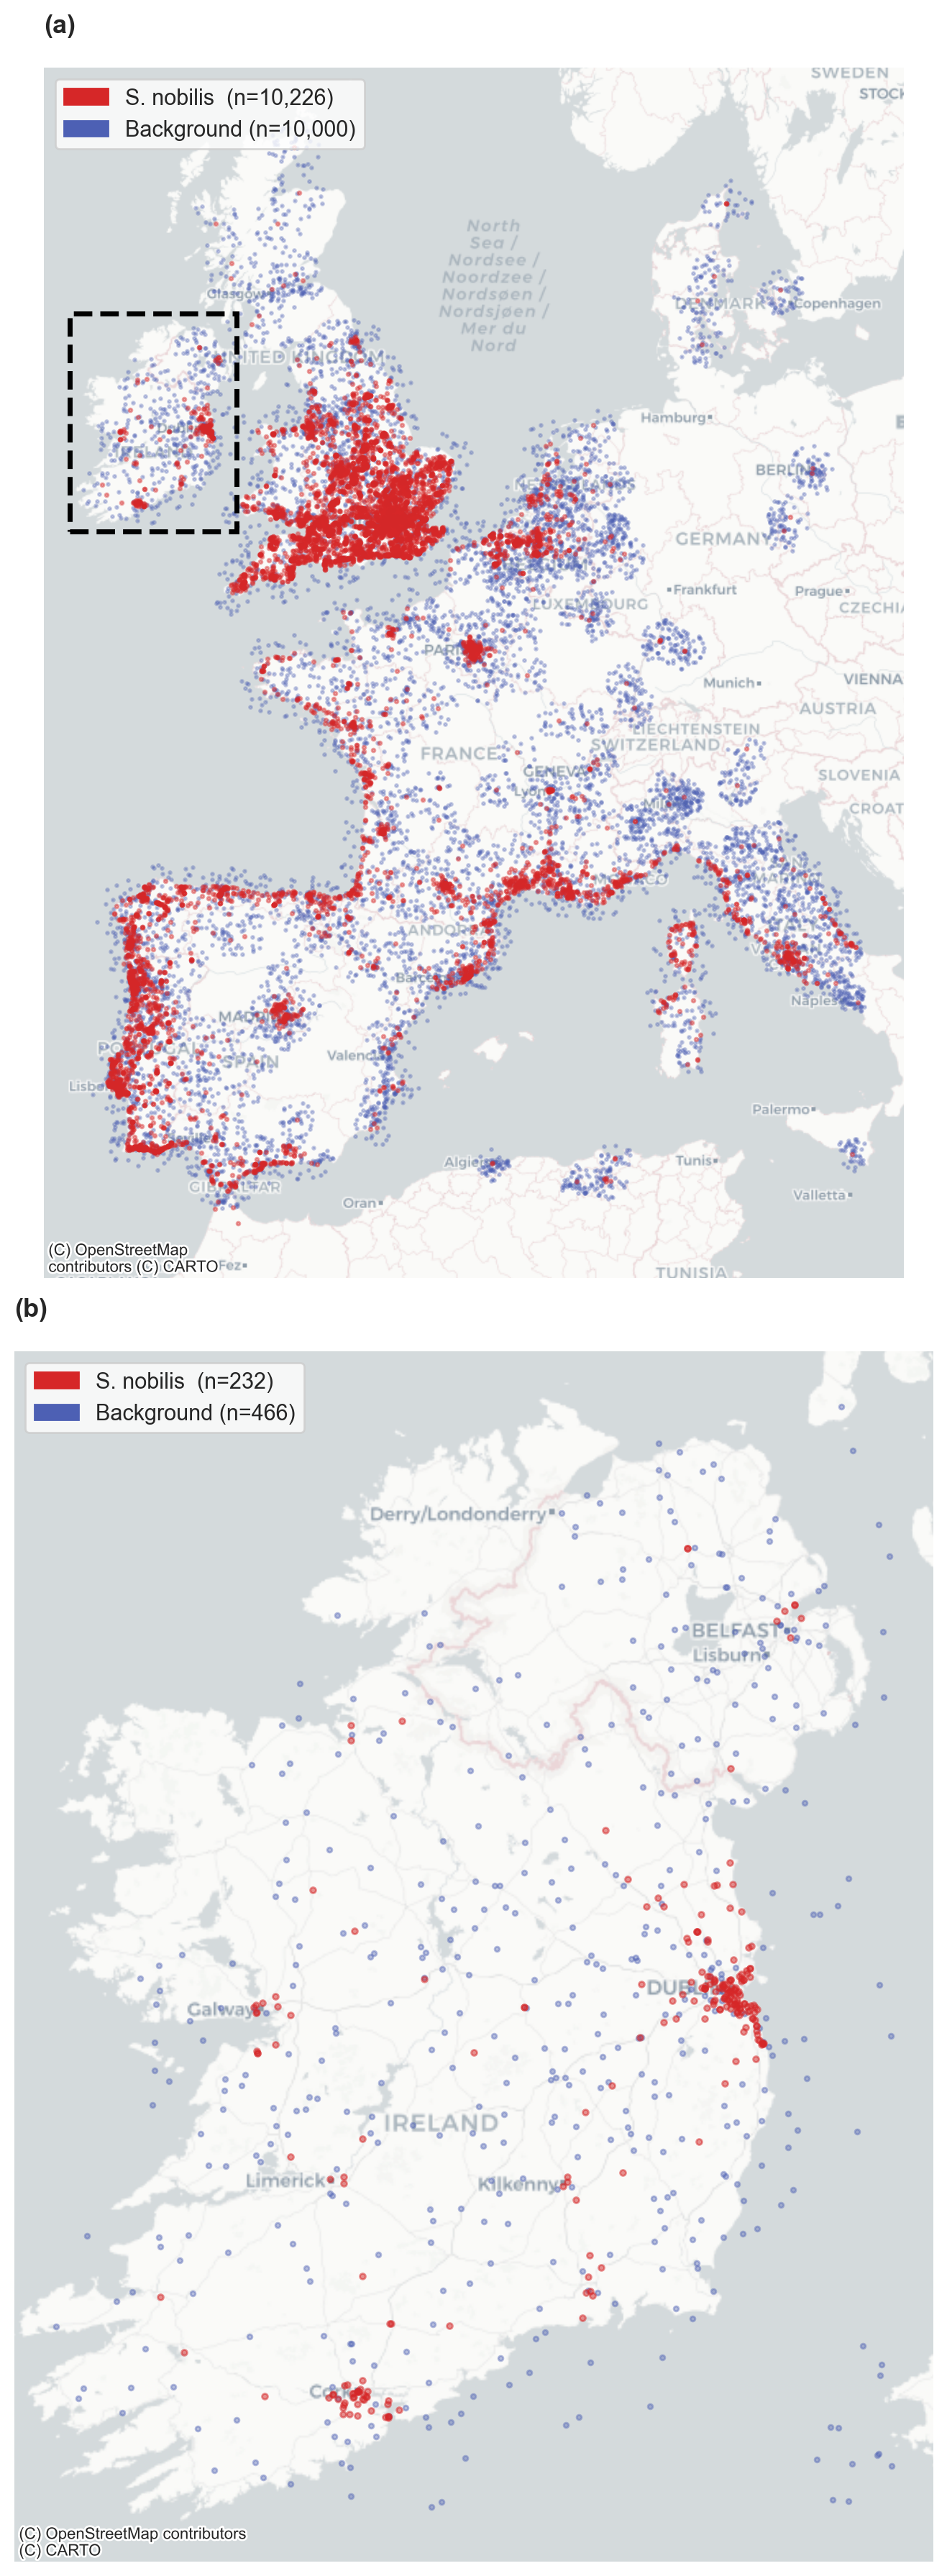
\includegraphics[width=0.9\columnwidth, trim=0 0 0 10]{../outputs/study_area_map.png}
\caption{(a) Distribution of \textit{Steatoda nobilis} occurrence records (red; $n = 10{,}226$) and bias-corrected pseudo-absence background points (grey; $n = 10{,}000$) across the Western European study area (35--60\textdegree N, 12\textdegree W--15\textdegree E). The dashed rectangle indicates the Ireland zoom region shown in panel~(b). Occurrences are concentrated in southern England, Ireland, northern France, and the Iberian Peninsula, reflecting the species' established range and citizen-science recording effort on iNaturalist and GBIF. (b) Ireland inset showing the 232 occurrence records concentrated around Dublin and the eastern seaboard, with scattered records in Cork, Limerick, and Belfast, alongside 466 bias-corrected background points.}
\label{fig:study_area_map}
\end{figure}

Because MaxEnt is a presence-background algorithm, it requires a set of background (pseudo-absence) points that characterise the environmental conditions available across the landscape \citep{Phillips2006, Elith2011}. To account for spatial bias in citizen-science recording effort, 10,000 background points were generated using a bias-corrected sampling scheme in which the probability of selecting a background location was proportional to the local density of all biodiversity records on iNaturalist within the study area \citep{Beck2014, Feldman2021}. This target-group approach ensures that the contrast between presence and background reflects genuine habitat preference rather than variation in recorder effort.

\subsection{Satellite environmental predictors}

Four satellite-derived environmental layers were produced using Google Earth Engine (GEE), chosen to capture two key dimensions of the species' synanthropic niche: artificial lighting and the thermal environment.

\textit{VIIRS nighttime radiance.} Monthly cloud-free composites from the Visible Infrared Imaging Radiometer Suite (VIIRS) Day/Night Band (DNB) were aggregated to a single median composite over 2017--2024 \citep{Elvidge2017}. The resulting layer represents the long-term average nighttime radiance in units of nW/cm$^{2}$/sr and serves as a direct proxy for the intensity of artificial light at night (ALAN) and, by extension, the degree of urbanisation.

\textit{MODIS daytime land surface temperature (LST).} Daytime LST observations from the MODIS Terra sensor (MOD11A2 Collection 6) were averaged across all available 8-day composites from 2017 to 2024 to produce a single annual mean layer in degrees Celsius \citep{Wan2014}. This variable captures the broadscale thermal environment at 1~km spatial resolution.

\textit{MODIS nighttime LST.} The nighttime component of the same MODIS product was processed identically to produce an annual mean nighttime LST layer. Nighttime LST is relevant to \textit{S.~nobilis} as a predominantly nocturnal species, and also reflects the degree of thermal buffering provided by urban infrastructure and heated buildings.

\textit{Landsat summer LST.} Surface temperature was derived from Landsat 8 and 9 Thermal Infrared Sensor (TIRS) Band 10 imagery acquired during June--August of 2017--2024. A median composite was calculated across the summer window to capture peak growing-season thermal conditions at a native resolution of 30~m, which was subsequently resampled to 1~km for the study area and 500~m for the Ireland-specific analysis.

All four layers were reprojected to EPSG:4326, resampled using bilinear interpolation, and co-registered to a common 1~km grid covering the full study area (3,000 $\times$ 2,778 pixels). A separate 500~m resolution stack was produced for Ireland (1,111 $\times$ 933 pixels) to enable finer-scale prediction. Environmental values were extracted at each occurrence and background location from the 1~km stack, yielding a combined presence--background dataset of 20,226 samples with four predictor columns. Rows with missing values (primarily points falling over water) were excluded, leaving 9,967 presence and 8,343 background samples for model training.

\section{Geospatial analysis and modelling}

\subsection{Artificial light and thermal analysis of habitat}

\begin{figure}[htbp]
\centering
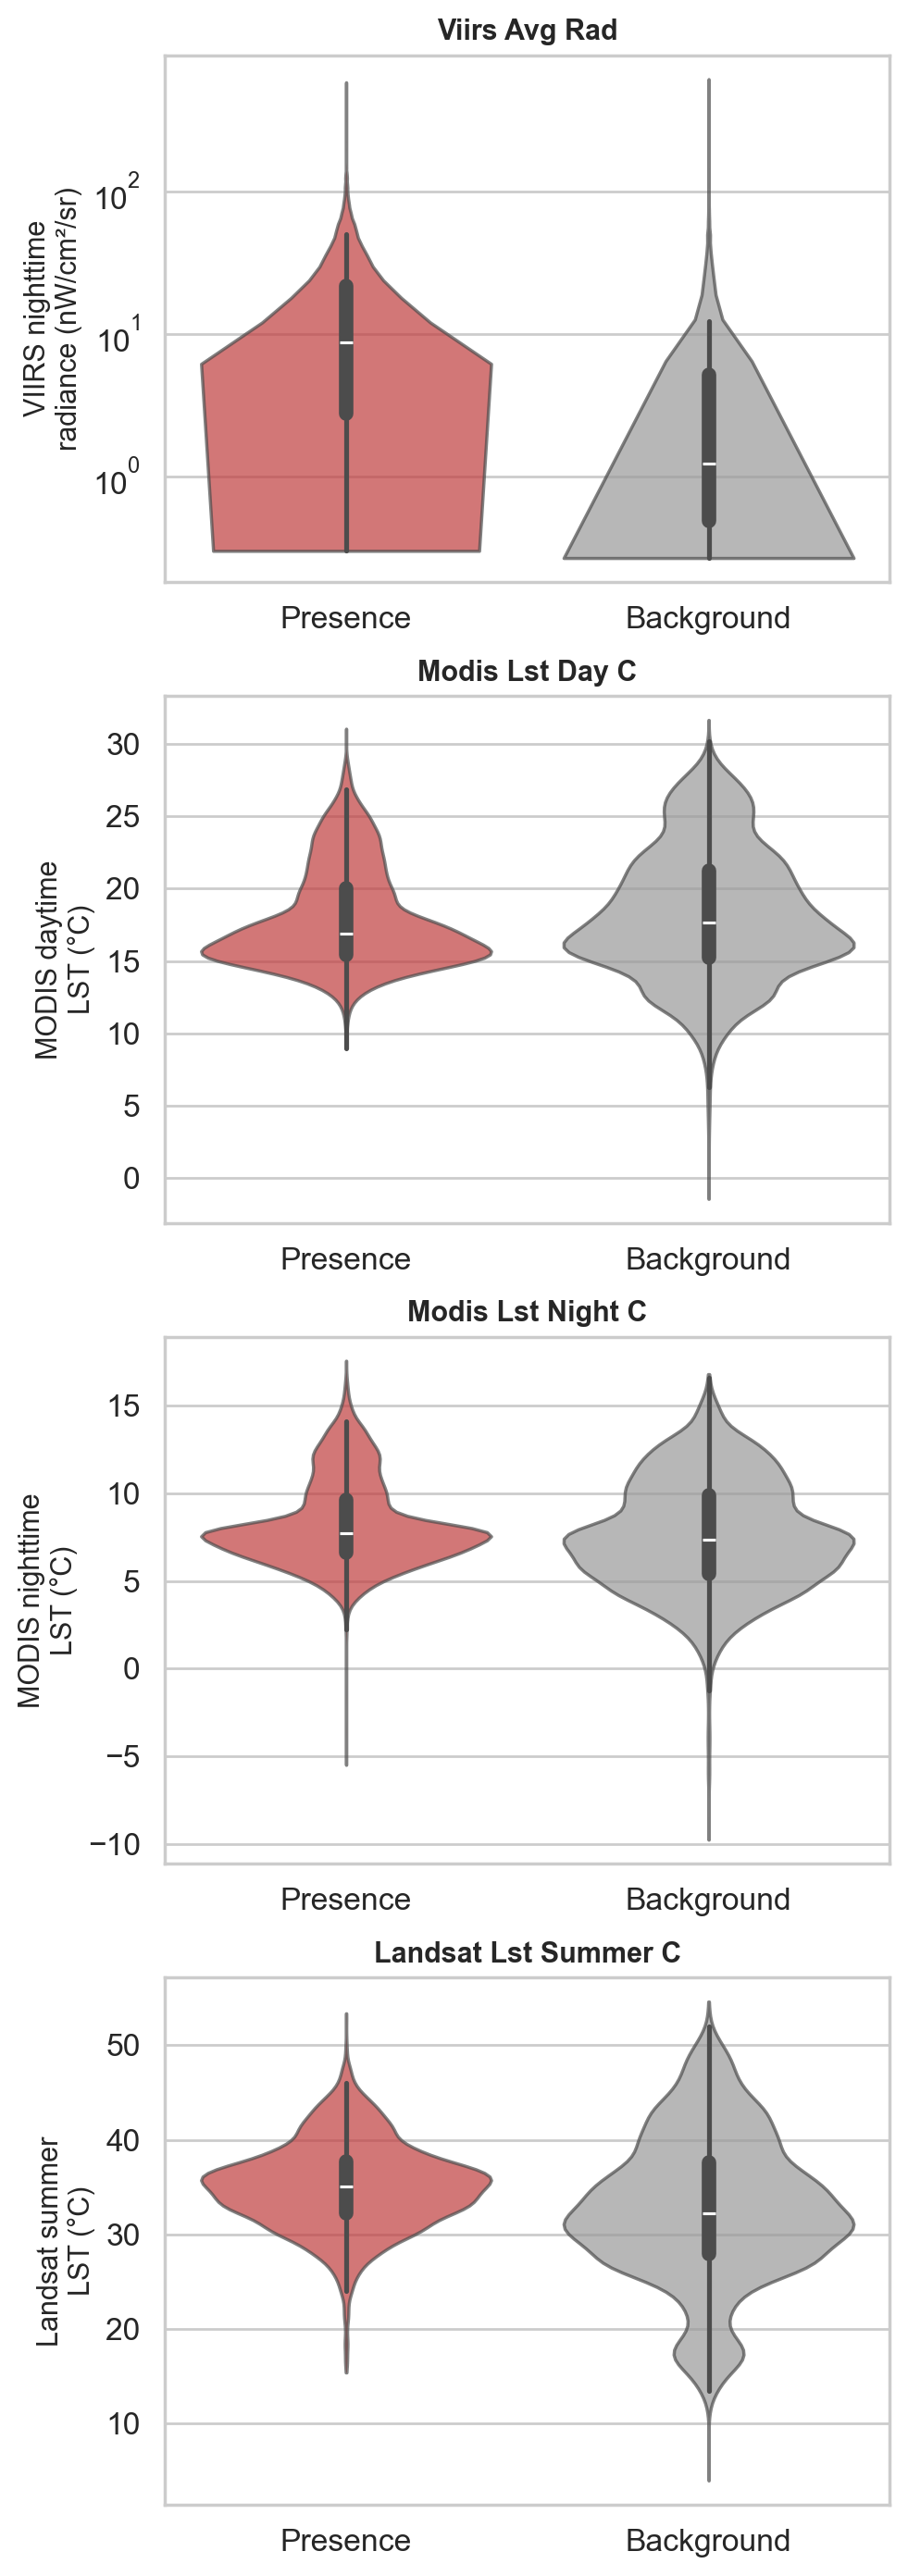
\includegraphics[width=0.78\columnwidth, trim= 20 0 0 0]{../outputs/violin_plots.png}
\caption{Violin plots comparing the distributions of four satellite-derived environmental variables at \textit{S.~nobilis} presence sites (red) versus pseudo-absence background locations (grey). Presence sites show markedly higher VIIRS nighttime radiance (median 8.7 vs 1.2~nW/cm\textsuperscript{2}/sr), confirming the species' association with artificially lit environments. Landsat summer LST is approximately 3\textdegree C warmer at presence sites (median 35.1 vs 32.3\textdegree C), while MODIS daytime and nighttime LST show narrower, warmer distributions for presences.}
\label{fig:violin_plots}
\end{figure}

Prior to model fitting, the distributions of the four satellite-derived predictor variables 
were compared between presence and background locations (Fig.~\ref{fig:violin_plots}). 
Presence sites exhibited substantially higher VIIRS nighttime radiance than background 
locations (median 8.7 vs 1.2~nW/cm$^{2}$/sr), confirming the species' strong association 
with artificially lit environments. Landsat summer LST was approximately 3\textdegree C warmer 
at presence sites (median 35.1\textdegree C vs 32.3\textdegree C), while MODIS daytime LST 
showed a narrower distribution centred on cooler temperate values for presences 
(median 13.8\textdegree C vs 15.2\textdegree C), consistent with the species' current 
concentration in maritime climates of the British Isles and Atlantic France rather than 
warmer Mediterranean regions. MODIS nighttime LST was slightly higher at presence sites 
(median 7.9\textdegree C vs 6.8\textdegree C).


Pairwise correlations among the three LST variables were moderate to high ($r = 0.65$--$0.85$), as expected for thermal variables derived from overlapping spectral and temporal windows. However, VIIRS nighttime radiance was only weakly correlated with each of the LST variables ($r = 0.25$--$0.34$), indicating that artificial light captures an independent environmental axis not redundant with the thermal predictors.


\subsection{MaxEnt spatial distribution modeling}

We used Maximum Entropy (MaxEnt) modelling, one of the most widely adopted algorithms for presence-only species distribution modelling \citep{Phillips2006, Phillips2008, Elith2011}. MaxEnt finds the probability distribution across environmental space that has maximum entropy (i.e.\ is closest to uniform) subject to the constraint that the expected values of environmental features at predicted presence sites must match their observed values at known occurrence locations. The principle of maximum entropy ensures that the model makes the fewest possible assumptions beyond what the data support, yielding the least biased estimate of the species' environmental niche \citep{Phillips2006}.

Formally, MaxEnt estimates a Gibbs distribution over environmental feature space:
\begin{equation}
f(\mathbf{z}) = \frac{\exp\!\bigl(\boldsymbol{\lambda} \cdot \mathbf{h}(\mathbf{z})\bigr)}{Z}
\label{eq:maxent}
\end{equation}
Here $\mathbf{z}$ is the vector of environmental variables measured at a site. In our case each location is described by four satellite-derived quantities:
\begin{equation}
\mathbf{z} = \begin{pmatrix} z_1 \\ z_2 \\ z_3 \\ z_4 \end{pmatrix} = \begin{pmatrix} \text{VIIRS nighttime radiance (nW\,cm}^{-2}\,\text{sr}^{-1}\text{)} \\ \text{MODIS daytime LST (\textdegree C)} \\ \text{MODIS nighttime LST (\textdegree C)} \\ \text{Landsat summer LST (\textdegree C)} \end{pmatrix}
\label{eq:zvec}
\end{equation}
so that, for example, a presence record in suburban Dublin might have $\mathbf{z} \approx (10.2,\; 16.9,\; 7.3,\; 29.5)^{T}$, while a rural background point in western Ireland might have $\mathbf{z} \approx (0.5,\; 14.1,\; 5.8,\; 24.3)^{T}$. The model learns which regions of this four-dimensional environmental space are preferentially occupied by the species.

$\mathbf{h}(\mathbf{z})$ is a vector of \emph{derived features} that allow non-linear and interactive responses. With our configuration (linear, hinge, and product features across four variables) the feature vector comprises $4 + 40 + 6 = 50$ elements:
\begin{equation}
\mathbf{h}(\mathbf{z}) = \bigl(\;\underbrace{z_1,\, z_2,\, z_3,\, z_4}_{4\;\text{linear}},\;\;\underbrace{h_{1}^{(1)}(z_1),\,\ldots,\,h_{10}^{(4)}(z_4)}_{40\;\text{hinge}},\;\;\underbrace{z_1 z_2,\, z_1 z_3,\, \ldots,\, z_3 z_4}_{6\;\text{product}}\;\bigr)^{T}
\label{eq:features}
\end{equation}
Each hinge feature is a piecewise-linear function with a knot at a threshold $\tau_k$:
\begin{equation}
h_k^{(j)}(z_j) = \max\!\bigl(0,\; z_j - \tau_k\bigr)
\label{eq:hinge}
\end{equation}
These act as soft switches that are zero below the threshold and increase linearly above it, enabling the model to capture abrupt environmental thresholds (e.g.\ suitability increasing sharply once nighttime temperature exceeds ${\sim}6$\textdegree C). Ten hinge knots are placed at evenly spaced quantiles across each variable's range.

$\boldsymbol{\lambda} = (\lambda_1, \ldots, \lambda_{50})^{T}$ are the learned feature weights: a positive $\lambda_i$ means higher values of feature $h_i$ increase predicted suitability, and vice versa. $Z = \sum_{\mathbf{z}} \exp(\boldsymbol{\lambda} \cdot \mathbf{h}(\mathbf{z}))$ is a normalising constant ensuring the distribution sums to unity over all landscape pixels.

The raw Gibbs output is a relative density, not a probability. It is transformed to the \textbf{complementary log-log (cloglog)} scale to produce a habitat suitability index on $[0, 1]$ \citep{Phillips2008}:
\begin{equation}
\text{suitability}(\mathbf{z}) = 1 - \exp\!\bigl(-\exp(\boldsymbol{\lambda} \cdot \mathbf{h}(\mathbf{z}) - c)\bigr)
\label{eq:cloglog}
\end{equation}
where $c$ is a normalisation constant estimated from the data. Under certain assumptions about the sampling process, this output approximates the probability of presence in a given cell.

The product features ($z_i z_j$ terms in Eq.~\ref{eq:features}) allow the model to capture synergistic effects --- for example, the influence of artificial light on suitability may depend on temperature, so that warm, well-lit areas are more suitable than either variable alone would predict.

\begin{figure}[htbp]
\centering
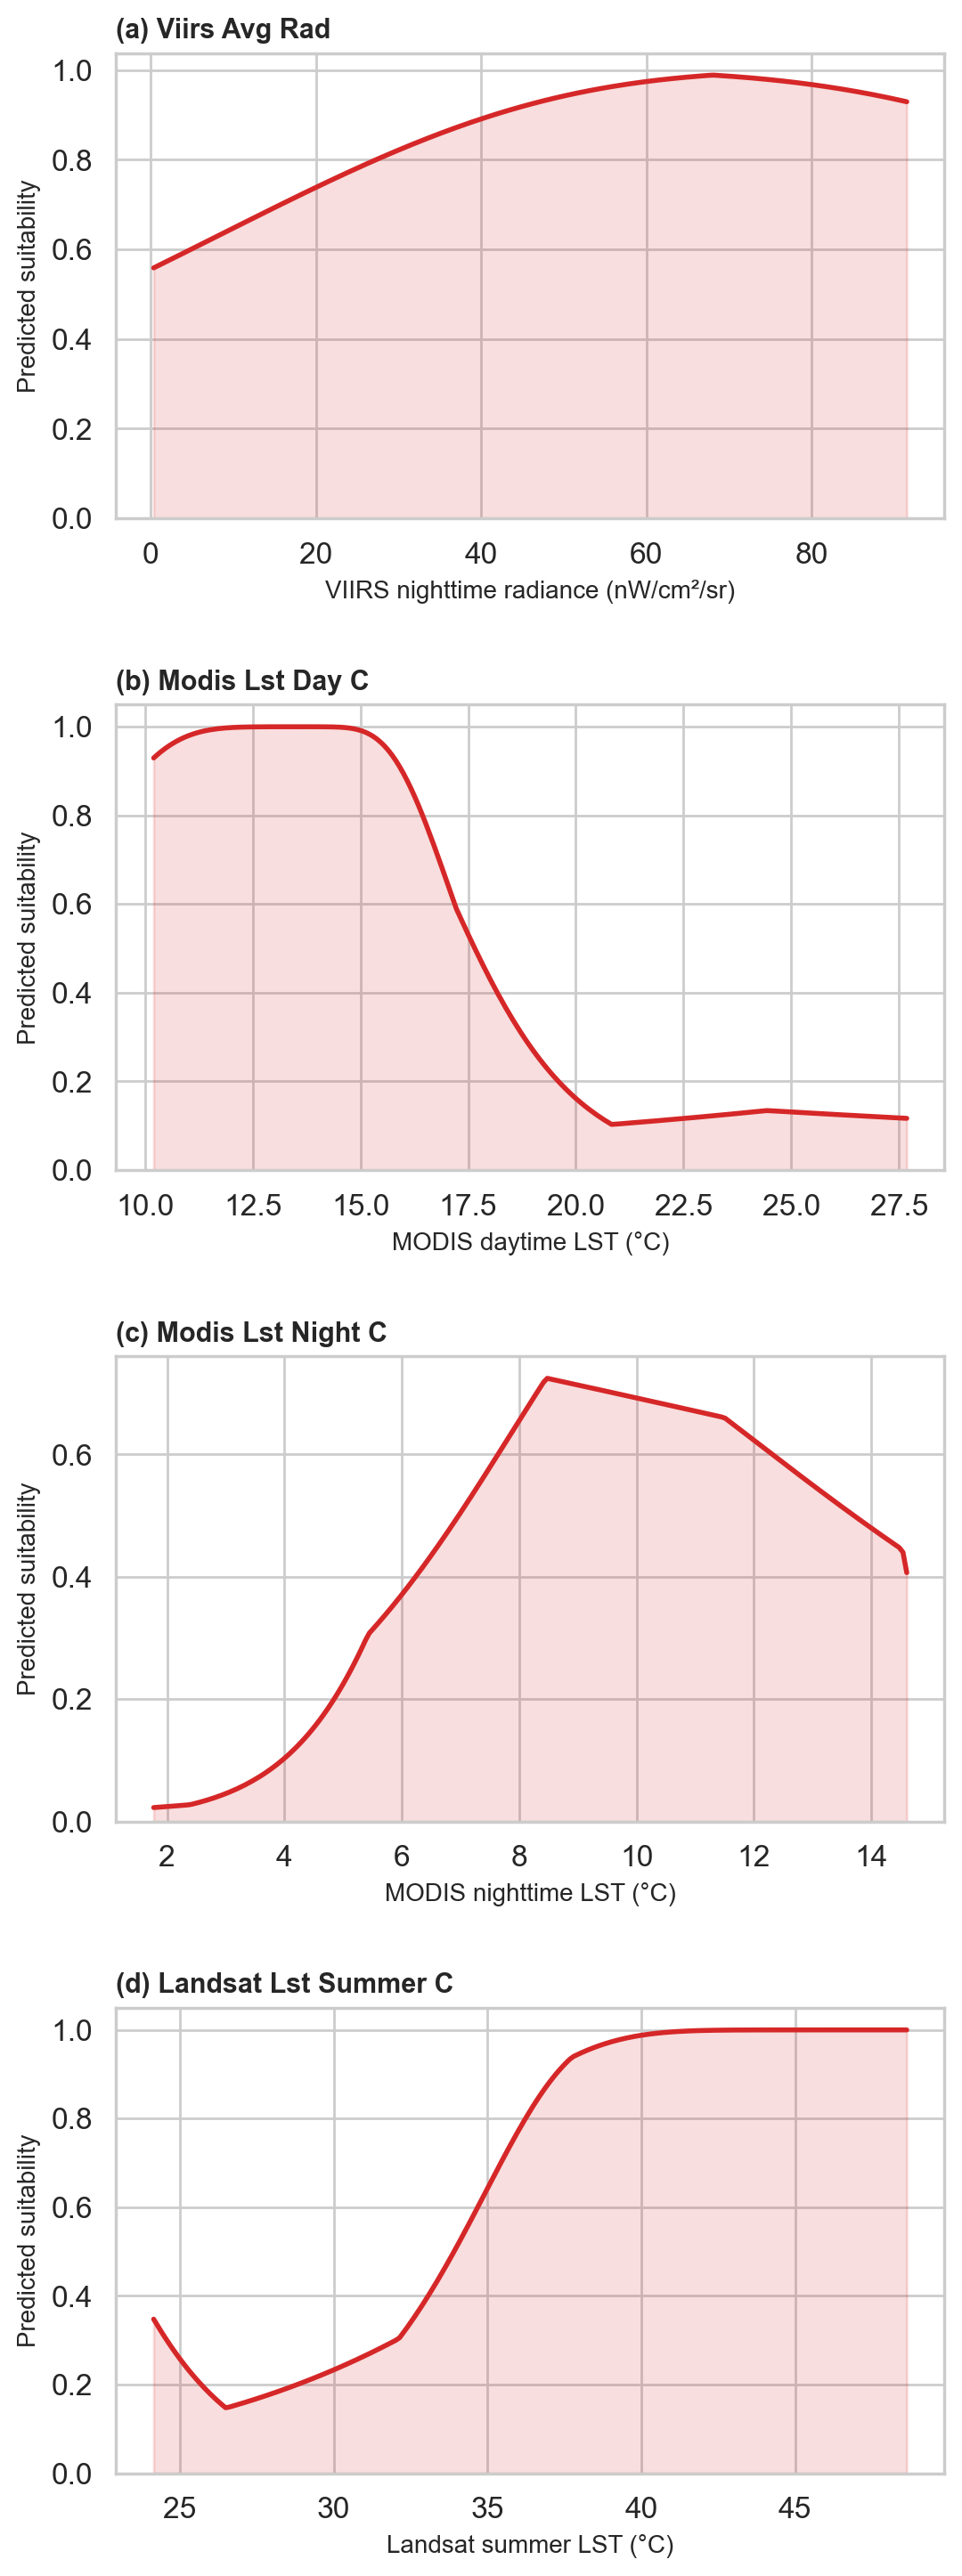
\includegraphics[width=0.85\columnwidth]{../outputs/response_curves.png}
\caption{Marginal response curves showing predicted habitat suitability as a function of each variable, with all other predictors held at their median values. (a) Suitability increases monotonically with VIIRS radiance. (b) MODIS daytime LST: suitability peaks at cooler values of 10--14\textdegree C. (c) MODIS nighttime LST: unimodal response peaking at 8--10\textdegree C. (d) Landsat summer LST: suitability increases above ${\sim}$30\textdegree C.}
\label{fig:response_curves}
\end{figure}

Model complexity was controlled by L1 (lasso) regularisation, scaled by a beta multiplier $\beta = 1.5$. The regularisation adds a penalty $\beta \sum_{i} |\lambda_i|$ to the log-likelihood (Eq.~\ref{eq:loglik} below), discouraging large weights on features that only marginally improve fit and thereby producing smoother, more generalisable response curves. We set $\beta$ above its default value of 1.0 following the recommendations of \citet{Merow2013}, who showed that moderate over-regularisation typically improves transferability with minimal loss in discriminatory power.

Importantly, MaxEnt is a \textit{presence--background} method: rather than requiring confirmed absences, it contrasts the environmental conditions at known occurrence sites against those sampled from the landscape as a whole (represented by the 10,000 bias-corrected background points described above). Formally, the model maximises the regularised log-likelihood:
\begin{equation}
\mathcal{L}(\boldsymbol{\lambda}) = \frac{1}{n}\sum_{i=1}^{n} \boldsymbol{\lambda} \cdot \mathbf{h}(\mathbf{z}_i) \;-\; \ln\!\Biggl(\frac{1}{m}\sum_{j=1}^{m} e^{\,\boldsymbol{\lambda}\cdot\mathbf{h}(\tilde{\mathbf{z}}_j)}\Biggr) \;-\; \beta\sum_{k}|\lambda_k|
\label{eq:loglik}
\end{equation}
where $\mathbf{z}_1, \ldots, \mathbf{z}_n$ are the $n = 9{,}967$ presence locations and $\tilde{\mathbf{z}}_1, \ldots, \tilde{\mathbf{z}}_m$ are the $m = 8{,}343$ background points. The first term rewards high predicted values at presence sites; the second penalises high predictions across the background (preventing the model from predicting high suitability everywhere); the third is the regularisation penalty.

The fitting procedure works as follows. Before optimisation begins, the 50 derived features $h_i(\mathbf{z})$ are constructed from the raw environmental variables using fixed, predetermined transformations: the four linear features are simply the raw values, the 40 hinge knots are placed at fixed quantiles of each variable's range, and the six product features are pairwise multiplications. Because these transformations are deterministic and do not depend on $\boldsymbol{\lambda}$, the feature values at every presence and background site are fully known prior to fitting. The target that the model must match is the \emph{mean of each feature evaluated at the presence sites}:
\begin{equation}
\bar{h}_i = \frac{1}{n}\sum_{j=1}^{n} h_i(\mathbf{z}_j)
\label{eq:empirical_mean}
\end{equation}
These are not raw observations but computed summaries of the environmental conditions at known occurrence locations. The maximum-entropy principle requires that the model's expected value of each feature --- computed as a weighted average over the background landscape --- must equal this presence-site mean. Setting the gradient of $\mathcal{L}$ to zero yields exactly this constraint: at the optimum, $\partial \mathcal{L}/\partial \lambda_i = 0$ implies
\begin{equation}
\bar{h}_i \;=\; \frac{\sum_{j=1}^{m} h_i(\tilde{\mathbf{z}}_j)\,\exp\!\bigl(\boldsymbol{\lambda}\cdot\mathbf{h}(\tilde{\mathbf{z}}_j)\bigr)}{\sum_{j=1}^{m} \exp\!\bigl(\boldsymbol{\lambda}\cdot\mathbf{h}(\tilde{\mathbf{z}}_j)\bigr)}
\label{eq:constraint}
\end{equation}
The left-hand side is a fixed quantity computed once from the presence data; the right-hand side is the model-weighted mean of the same feature across the background, which changes as $\boldsymbol{\lambda}$ is updated. The optimisation adjusts $\boldsymbol{\lambda}$ until these two sides agree for every feature simultaneously (up to the regularisation penalty, which relaxes the matching for weakly informative features by shrinking the corresponding $\lambda_i$ toward zero). To give a concrete example: presence sites have a mean VIIRS radiance of ${\sim}$16.6~nW\,cm$^{-2}$\,sr$^{-1}$, far above the background mean of ${\sim}$6.1. The model must therefore assign higher weights to brighter background pixels --- increasing $\lambda_1$ --- until the model-weighted mean radiance across the landscape rises to match ${\sim}$16.6, or as close to it as the regularisation allows.

The weight vector $\boldsymbol{\lambda}$ is optimised iteratively using the L-BFGS-B algorithm \citep{Byrd1995}, a quasi-Newton method that approximates the Hessian matrix from successive gradient evaluations. Starting from $\boldsymbol{\lambda} = \mathbf{0}$ (which corresponds to a uniform distribution, assigning equal suitability everywhere), the algorithm iteratively updates the weights in the direction that most steeply increases $\mathcal{L}$, converging when the gradient is sufficiently close to zero. Because Eq.~\ref{eq:loglik} is concave in $\boldsymbol{\lambda}$, the optimum is unique and the algorithm is guaranteed to converge to the global maximum.

The model therefore learns what distinguishes presence sites from the available environmental background, not from locations where the species is known to be absent --- a key advantage for citizen-science datasets where non-detection does not imply true absence \citep{Elith2011}.

The model was implemented using the \texttt{elapid} Python package, which provides a scikit-learn-compatible MaxEnt implementation with native support for geographic cross-validation and raster prediction. It was trained on the full presence--background dataset (9,967 presences, 8,343 background samples) with the four satellite-derived predictors described above.

Variable importance was assessed using permutation importance, in which each predictor was randomly shuffled 10 times and the resulting mean drop in the area under the receiver operating characteristic curve (AUC) was recorded. This approach evaluates each variable's contribution to model performance on the full dataset after fitting, providing a more stable assessment than MaxEnt's built-in training-time contribution metrics, which can be sensitive to the order in which variables are added \citep{Elith2011}. Marginal response curves were generated by varying each predictor across its observed range while holding all other variables at their median values, providing partial-dependence plots that isolate each variable's individual effect on predicted suitability.

The trained model was applied to the full raster stacks to generate continuous habitat suitability surfaces (range 0--1) for the Western European study area at 1~km resolution and for Ireland at 500~m resolution.

\begin{figure}[htbp]
\centering
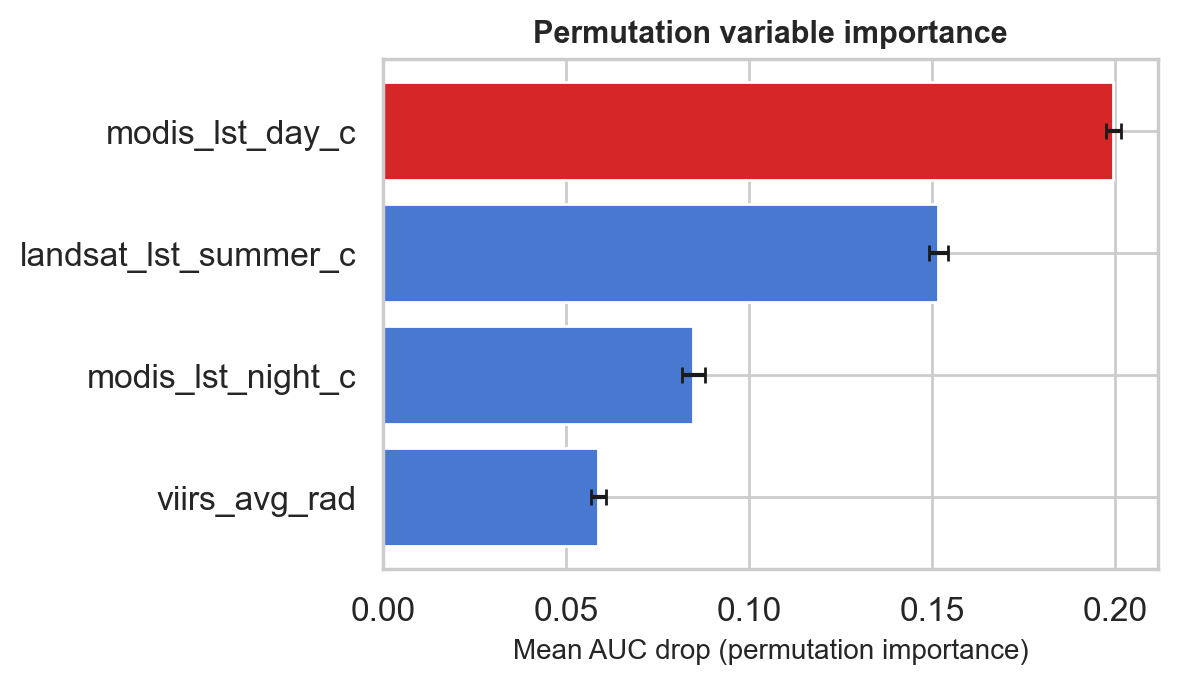
\includegraphics[width=0.85\columnwidth]{../outputs/variable_importance.png}
\caption{Permutation importance of the four satellite-derived predictors, measured as the mean drop in AUC ($\pm$ s.d.) when each variable is randomly shuffled (10 permutations). MODIS daytime LST is the strongest predictor (AUC drop = 0.20), followed by Landsat summer LST (0.15), MODIS nighttime LST (0.09), and VIIRS nighttime radiance (0.06).}
\label{fig:variable_importance}
\end{figure}

\subsection{Spatial cross-validation}

Standard random cross-validation tends to produce optimistic estimates of model performance when occurrence data are spatially autocorrelated, because nearby training and test points share similar environmental conditions \citep{Roberts2017}. To obtain a more realistic assessment, we used 4-fold spatially blocked cross-validation implemented via the \texttt{GeographicKFold} class in \texttt{elapid}, which partitions the study area into spatially contiguous blocks such that all records within a block are assigned to the same fold \citep{Valavi2019}. In each fold, three blocks were used for training and the held-out block for testing. Model discrimination was evaluated using the area under the receiver operating characteristic curve (AUC). The ROC curve is constructed by plotting the true positive rate (sensitivity) against the false positive rate (1~$-$~specificity) across all possible classification thresholds. The AUC summarises this curve as a single scalar: it equals the probability that a randomly chosen presence site is assigned a higher predicted suitability than a randomly chosen background point. An AUC of 0.5 indicates discrimination no better than random, while a value of 1.0 indicates perfect separation of presence and background conditions. In the presence--background setting used here, the ``false positive rate'' refers to the fraction of background points incorrectly ranked above a given threshold, rather than confirmed absences, so AUC should be interpreted as a measure of the model's ability to distinguish occupied environments from the landscape as a whole rather than from places where the species is known to be absent \citep{Phillips2006, Elith2011}. Values above ${\sim}$0.7 are generally considered to indicate useful discrimination for presence--background models \citep{Elith2006}. AUC was calculated separately for each fold and reported as the mean $\pm$ standard deviation across the four folds.

\subsection{Model performance and variable importance}

The MaxEnt model achieved a training AUC of 0.80 on the full dataset. Under spatially blocked 4-fold cross-validation, the mean AUC was 0.69 ($\pm$ 0.03). The drop from training to cross-validated AUC is expected when spatial autocorrelation is present in the data: nearby points share similar environmental conditions, so random holdout schemes overestimate transferability \citep{Roberts2017}. A spatially cross-validated AUC of 0.69 indicates moderate but genuine discriminatory ability, particularly given that the model relies on only four satellite-derived predictors across a large and environmentally heterogeneous study area.

Permutation importance analysis revealed a clear hierarchy among predictors (Fig.~\ref{fig:variable_importance}). MODIS daytime LST was the single most important variable, with a mean AUC drop of 0.200 when shuffled, followed by Landsat summer LST (0.152), MODIS nighttime LST (0.085), and VIIRS nighttime radiance (0.059). Temperature variables thus collectively dominate model performance, accounting for the majority of the explained variation in habitat suitability. VIIRS radiance contributes a smaller but distinct and non-redundant signal, consistent with the low correlation between ALAN and LST identified in the exploratory analysis.

\begin{figure}[htbp]
\centering
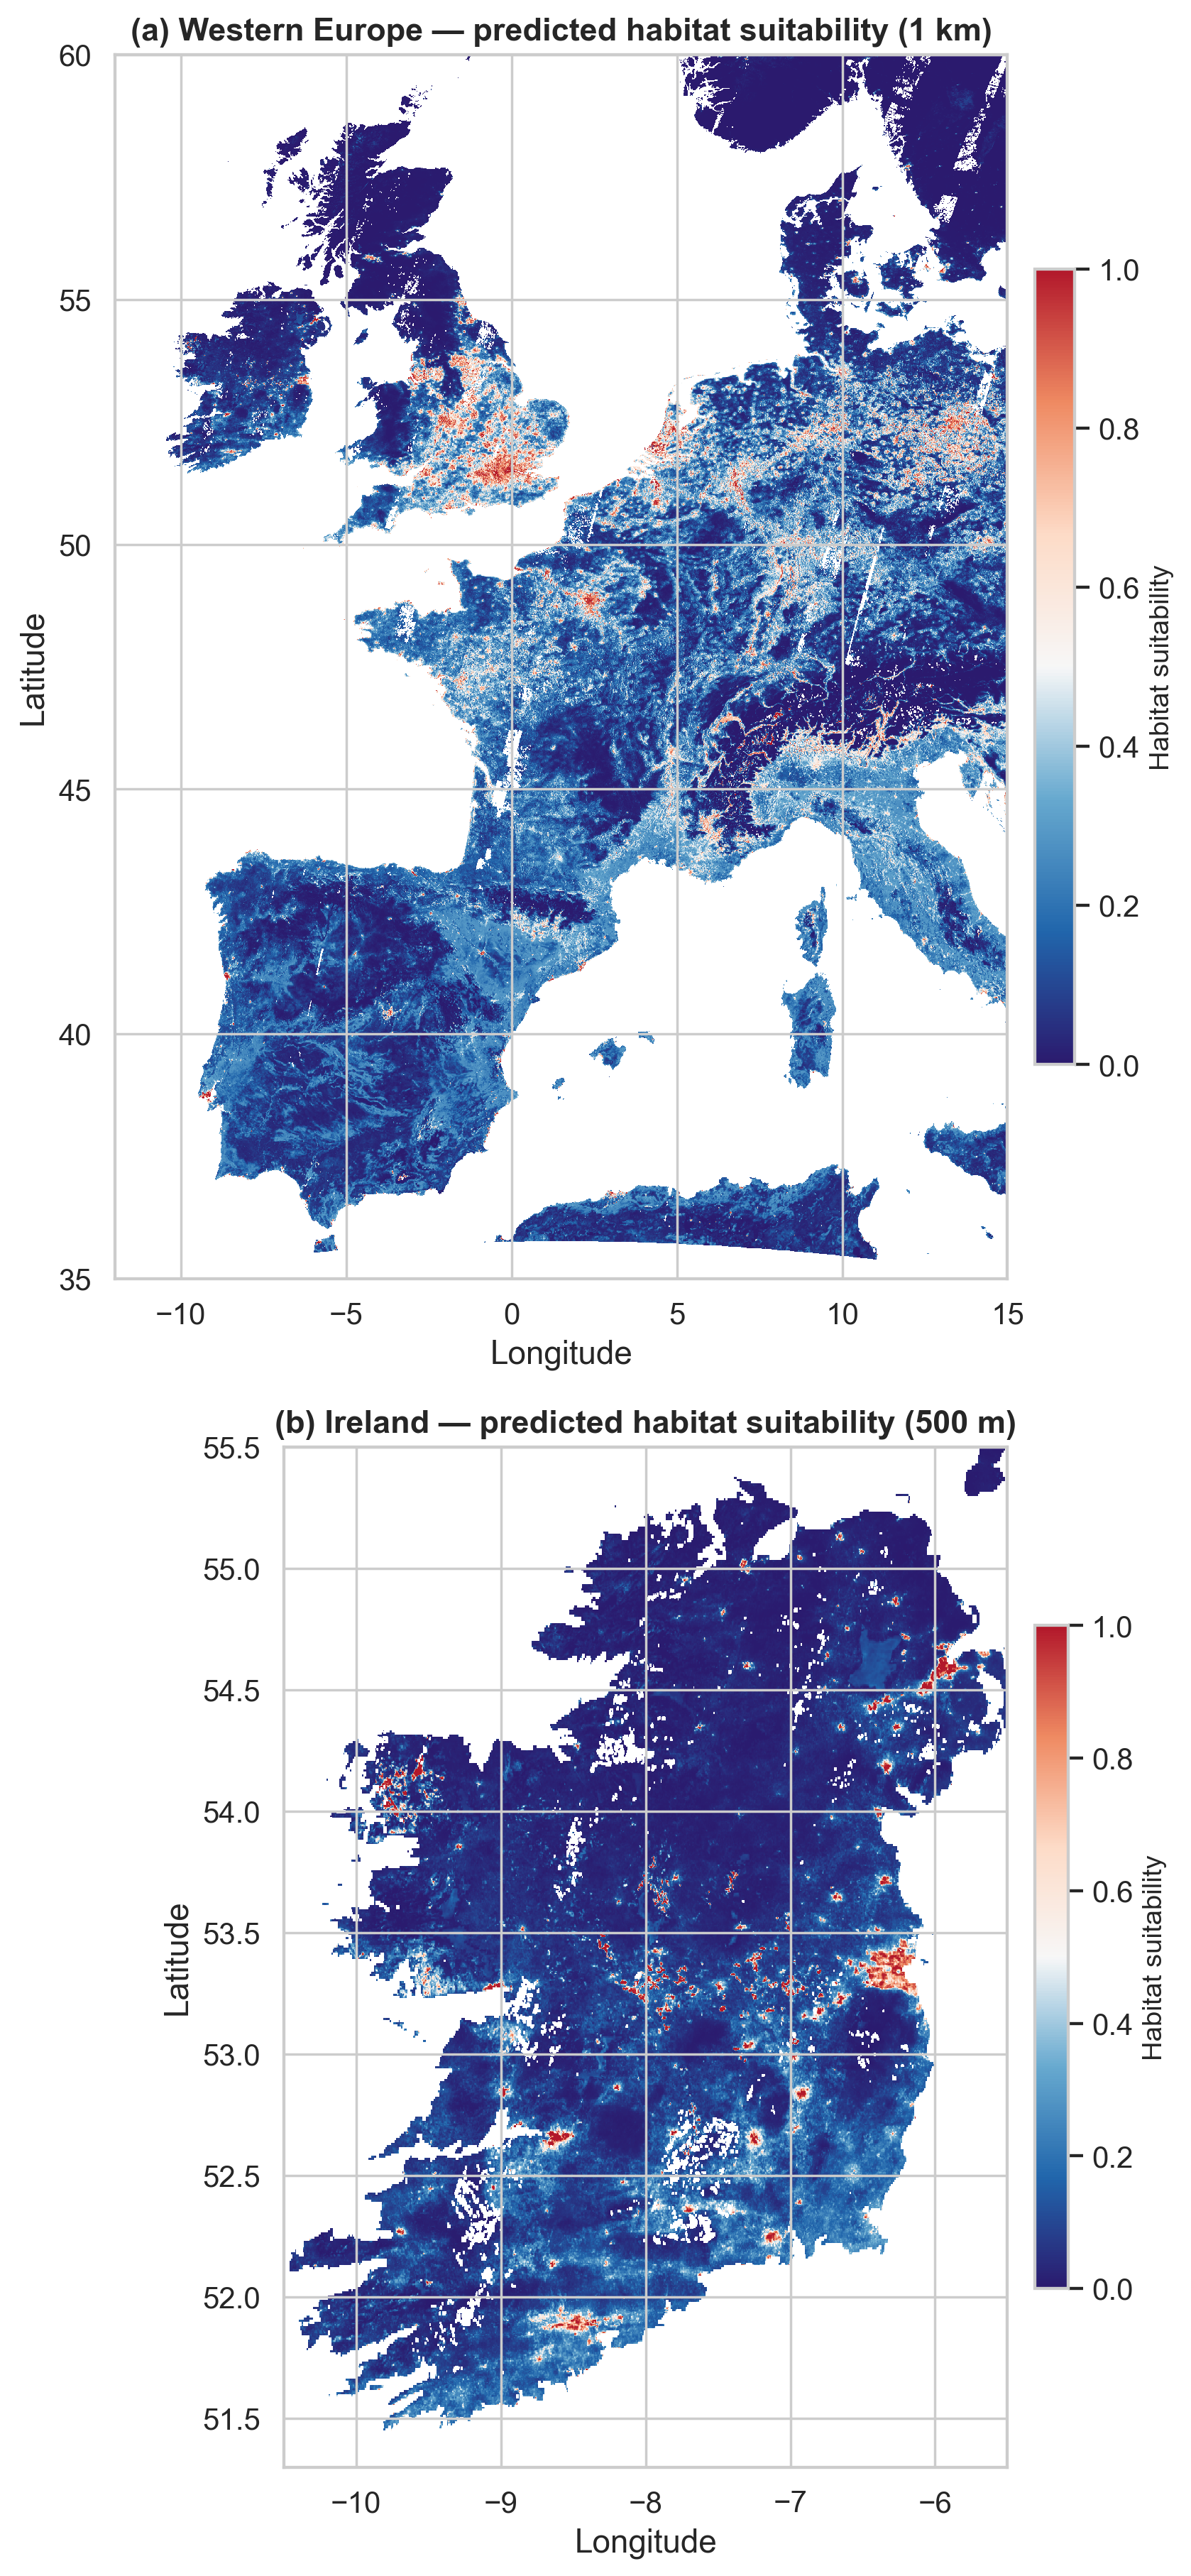
\includegraphics[width=\columnwidth]{../outputs/suitability_map_combined.png}
\caption{Predicted habitat suitability for \textit{S.~nobilis}. (a) Western Europe at 1~km resolution: highest suitability is predicted in southeastern England, the greater London area, northern France, and major urban centres, reflecting the species' dependence on warm, artificially lit built environments. (b) Ireland at 500~m resolution: elevated suitability is concentrated around Dublin, Cork, Limerick, Galway, Waterford, and Belfast; rural areas in the west and midlands show lower suitability. Both panels share the same 0--1 suitability colour scale derived from the MaxEnt model trained on VIIRS nighttime radiance, MODIS daytime and nighttime LST, and Landsat summer LST.}
\label{fig:suitability_maps}
\end{figure}

Marginal response curves illustrate the shape of the modelled relationships between each predictor and habitat suitability (Fig.~\ref{fig:response_curves}). Predicted suitability increases monotonically with VIIRS nighttime radiance, rising steeply below ${\sim}$20~nW/cm$^{2}$/sr and saturating above ${\sim}$60~nW/cm$^{2}$/sr. For MODIS daytime LST, suitability is highest at cooler values of 10--14\textdegree C and declines sharply above ${\sim}$18\textdegree C, reflecting the species' current core range in the mild maritime climates of the British Isles and Atlantic France rather than in warmer Mediterranean regions. MODIS nighttime LST shows a unimodal response peaking at 8--10\textdegree C, consistent with the moderate nocturnal temperatures typical of maritime urban environments. Landsat summer LST exhibits increasing suitability above ${\sim}$30\textdegree C, capturing the localised warming associated with built-up surfaces during the summer months.

\subsection{Predicted habitat suitability}

The trained model was applied to the full 1~km raster stack to produce a continuous habitat suitability surface across Western Europe (Fig.~\ref{fig:suitability_maps}a). The highest predicted suitability was concentrated in southeastern England --- particularly the greater London area and surrounding counties --- where the combination of high ALAN, moderate daytime LST, and warm summer surface temperatures closely matches the species' modelled niche. Northern France, including the Paris basin and the coastal strip from Normandy to Brittany, also showed elevated suitability. Across the wider study area, urban centres such as Brussels, Amsterdam, and cities along the Rhine corridor appeared as localised hotspots against a background of lower rural suitability. The Iberian Peninsula, despite being part of the species' native range, showed moderate rather than high suitability in many areas, likely because mean daytime LST in much of Iberia exceeds the optimal range identified by the model (10--14\textdegree C).

The 500~m resolution suitability surface for Ireland (Fig.~\ref{fig:suitability_maps}b) revealed a clear urban--rural gradient. Dublin and its surrounding commuter belt showed the highest predicted suitability on the island, followed by Cork, Limerick, Galway, Waterford, and Belfast. Smaller regional towns such as Kilkenny, Wexford, Drogheda, and Athlone were also visible as localised pockets of elevated suitability. Rural areas, particularly in the west and northwest, showed consistently low suitability values, reflecting lower ALAN and cooler summer LST. The finer spatial resolution of the Ireland stack (500~m vs 1~km) allowed individual towns and suburban areas to be resolved more clearly than in the study-area map.

\section{Temporal analysis}

\subsection{Logistic growth model}

To characterise the rate and trajectory of range expansion in Ireland, we overlaid all Irish occurrence records onto a grid of ${\sim}$10~km cells (0.1\textdegree\ $\times$ 0.1\textdegree) and tracked the cumulative number of unique cells occupied per year from 2017 to 2025. A three-parameter logistic growth model of the form

\begin{equation}
N(t) = \frac{K}{1 + e^{-r(t - t_0)}}
\label{eq:logistic}
\end{equation}

\noindent was fitted to the annual cumulative colonisation data using non-linear least squares (\texttt{scipy.optimize.curve\_fit}), where $K$ is the carrying capacity (maximum number of grid cells the species is expected to occupy), $r$ is the intrinsic rate of geographic spread, and $t_0$ is the inflection year at which the rate of colonisation is highest \citep{Verhulst1838, Shigesada1995}. The logistic model was projected forward to 2035 to estimate the timeline for 75\% and 90\% range saturation.

The predicted habitat suitability surface for Ireland (500~m) was aggregated to the same ${\sim}$10~km grid by computing the mean suitability per cell. Cells with mean suitability $\geq$ 0.4 but no occurrence records were flagged as high-suitability uncolonised cells, representing candidate locations for future establishment and priority targets for surveillance.

\subsection{Expansion in Ireland}

Annual \textit{S.~nobilis} sightings in Ireland increased from 2 in 2017 to 44 in 2025 (Fig.~\ref{fig:temporal}a), reflecting both genuine range expansion and growing public awareness and recording effort. Across the full study area, total annual records rose from 91 to 2,705 over the same period. To separate spatial spread from reporting intensity, we tracked the cumulative number of unique ${\sim}$10~km grid cells occupied over time. This metric grew from 2 cells in 2017 to 85 cells by 2025, indicating sustained geographic expansion across the island.

\begin{figure}[htbp]
\centering
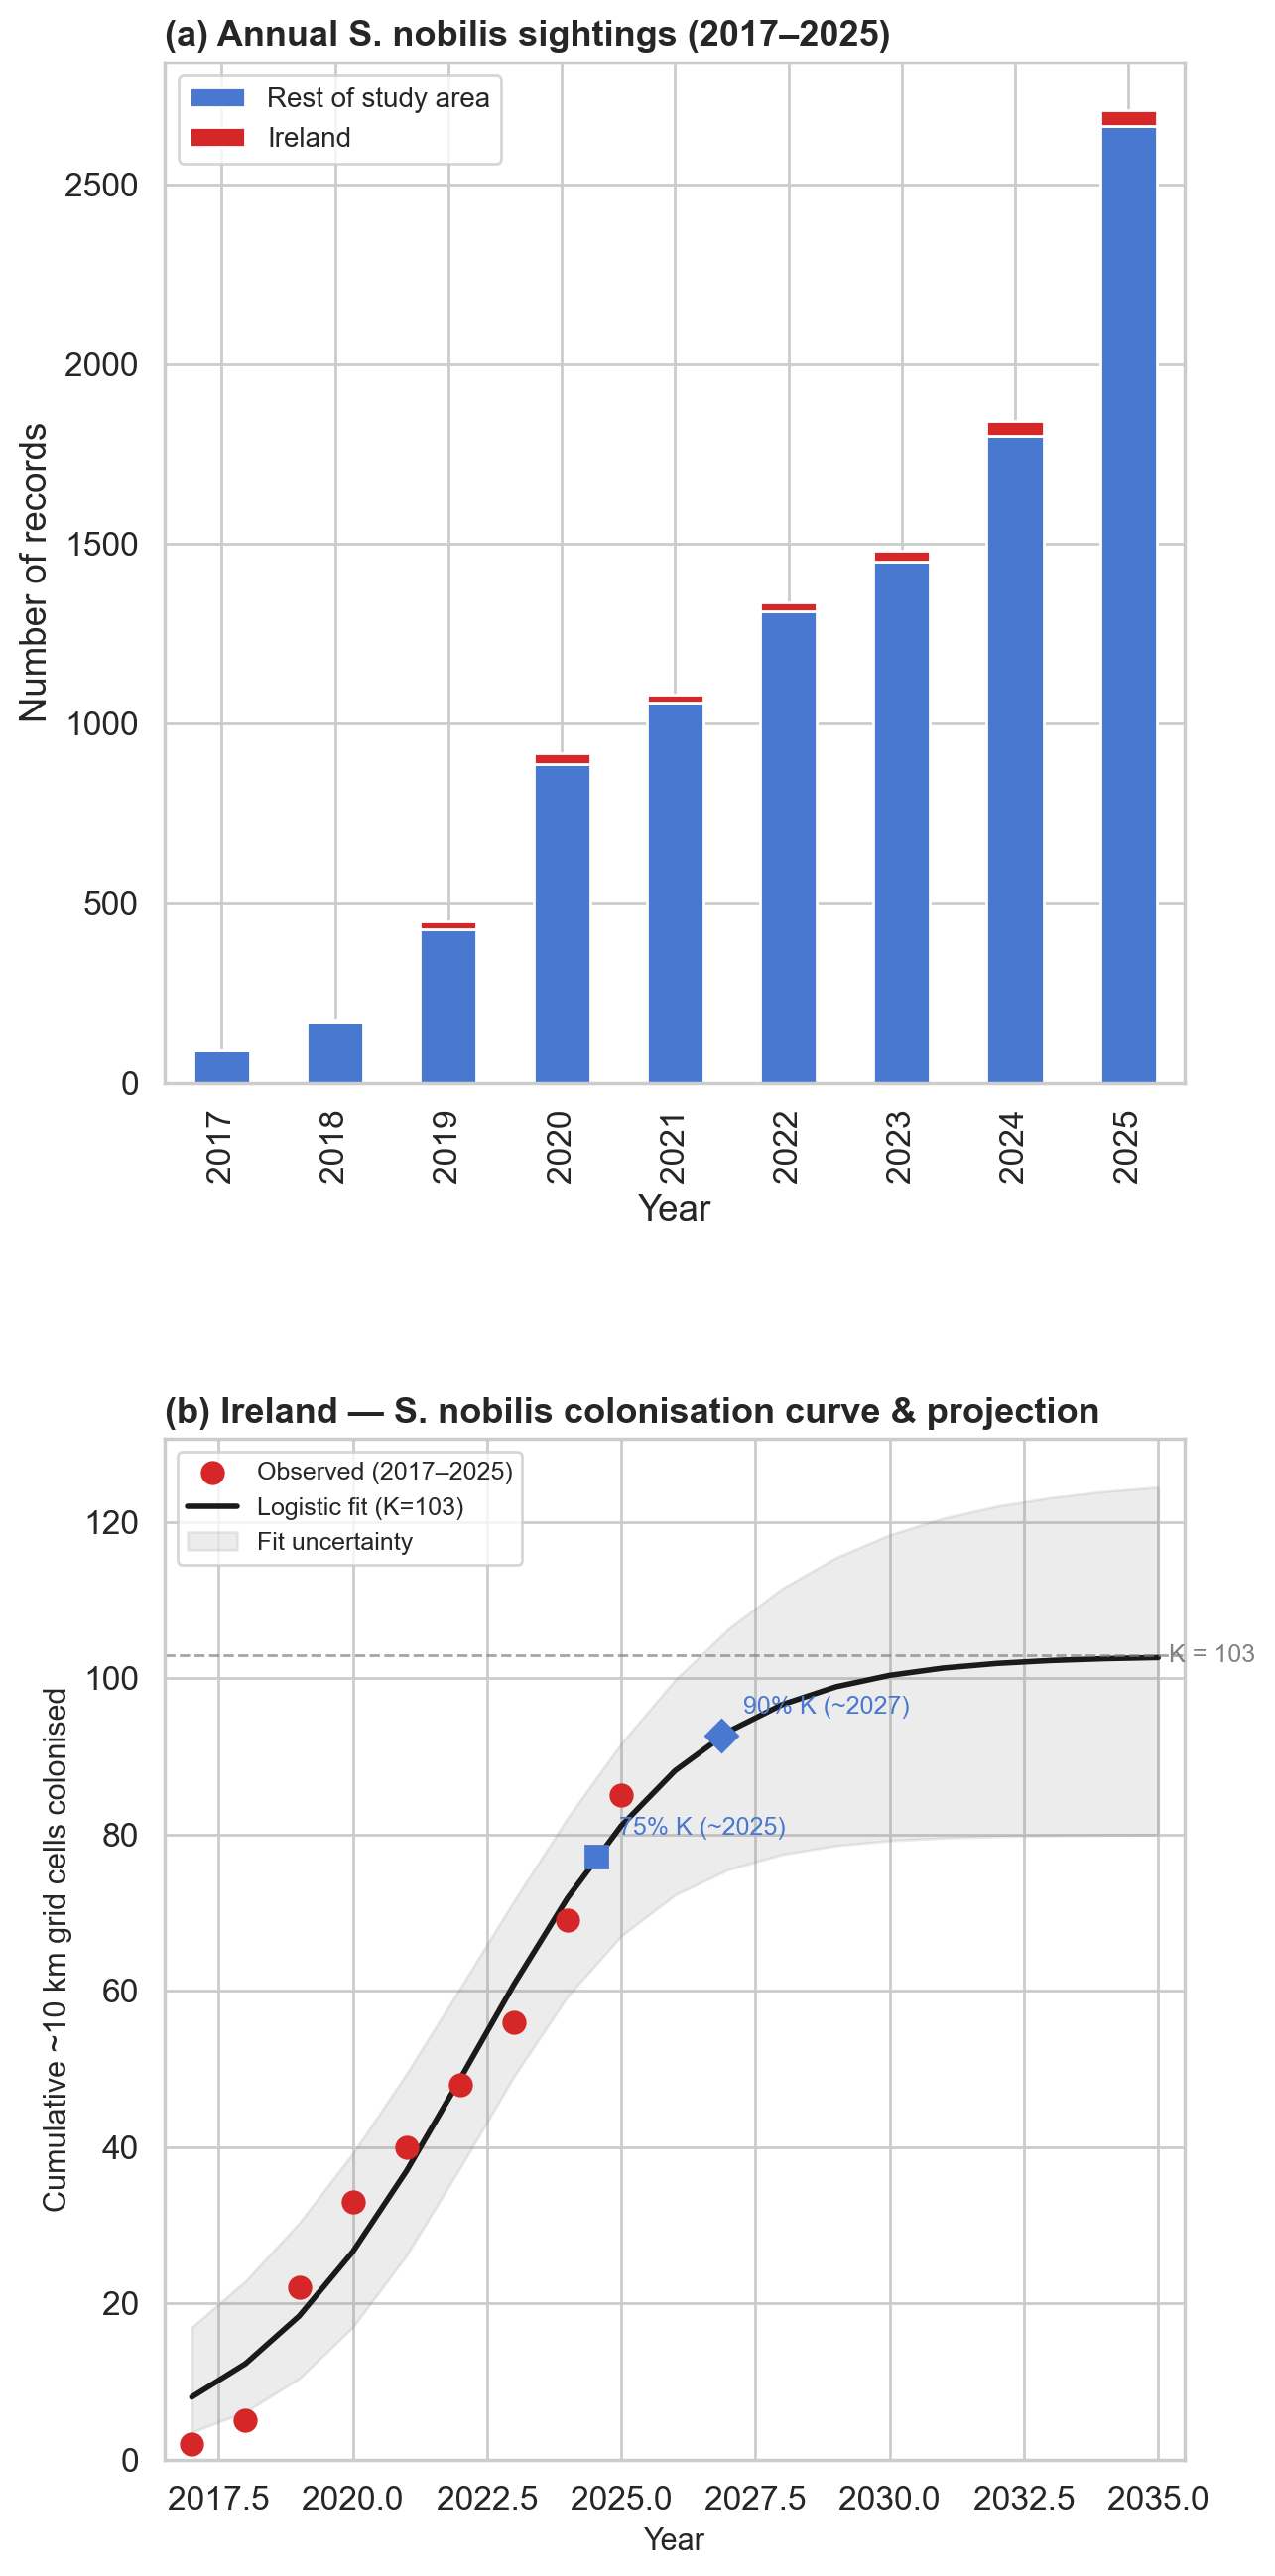
\includegraphics[width=\columnwidth]{../outputs/temporal_combined.png}
\caption{Temporal trends in \textit{S.~nobilis} occurrence and geographic spread. (a) Annual sighting records from 2017 to 2025 for the full study area (blue) and Ireland (red); total records increased more than 30-fold over this period, reflecting both genuine range expansion and growing citizen-science participation. (b) Cumulative geographic spread in Ireland measured as the number of unique ${\sim}$10~km grid cells with at least one record per year (red circles). A logistic growth model (black curve; grey shading = fit uncertainty) estimates a carrying capacity of $K = 103$ grid cells ($\pm$ 23), a growth rate of $r = 0.47$~yr$^{-1}$, and an inflection year of 2022. The model projects 75\% of $K$ reached by ${\sim}$2025 (blue square) and 90\% by ${\sim}$2027 (blue diamond), indicating the species is approaching range saturation in Ireland.}
\label{fig:temporal}
\end{figure}

A logistic growth model (Eq.~\ref{eq:logistic}) fitted to the cumulative colonisation curve provided a close fit to the observed data (Fig.~\ref{fig:temporal}b). The estimated carrying capacity was $K = 103$ grid cells ($\pm$ 23), with an intrinsic growth rate of $r = 0.47$~yr$^{-1}$ and an inflection year of $t_0 = 2022$, corresponding to the period of most rapid geographic spread. According to the fitted model, the species reached approximately 75\% of its estimated carrying capacity by ${\sim}$2025 and is projected to reach 90\% by ${\sim}$2027. These projections suggest that \textit{S.~nobilis} is entering the decelerating phase of range filling in Ireland, with most suitable habitat already colonised.

To identify where the remaining expansion is most likely to occur, we compared the set of already-colonised grid cells ($n = 72$ cells with $\geq$1 record as of 2025) against cells with high predicted suitability ($\geq$ 0.4) but no records to date (Fig.~\ref{fig:uncolonised_suitable}). A total of 34 high-suitability uncolonised cells were identified, concentrated in the Irish midlands and in regional towns with moderate urban development but relatively low citizen-science recorder activity. The top candidate areas for future colonisation include the Tullamore--Athlone corridor in the midlands, the greater Waterford area, Naas and surrounding County Kildare, the Ennis--Shannon area in County Clare, Navan in County Meath, and the Dundalk--Newry cross-border region. These locations share common characteristics: moderate levels of artificial lighting, proximity to existing colonised cells, and the presence of residential and commercial buildings that provide the heated structures favoured by the species.

\begin{figure}[htbp]
\centering
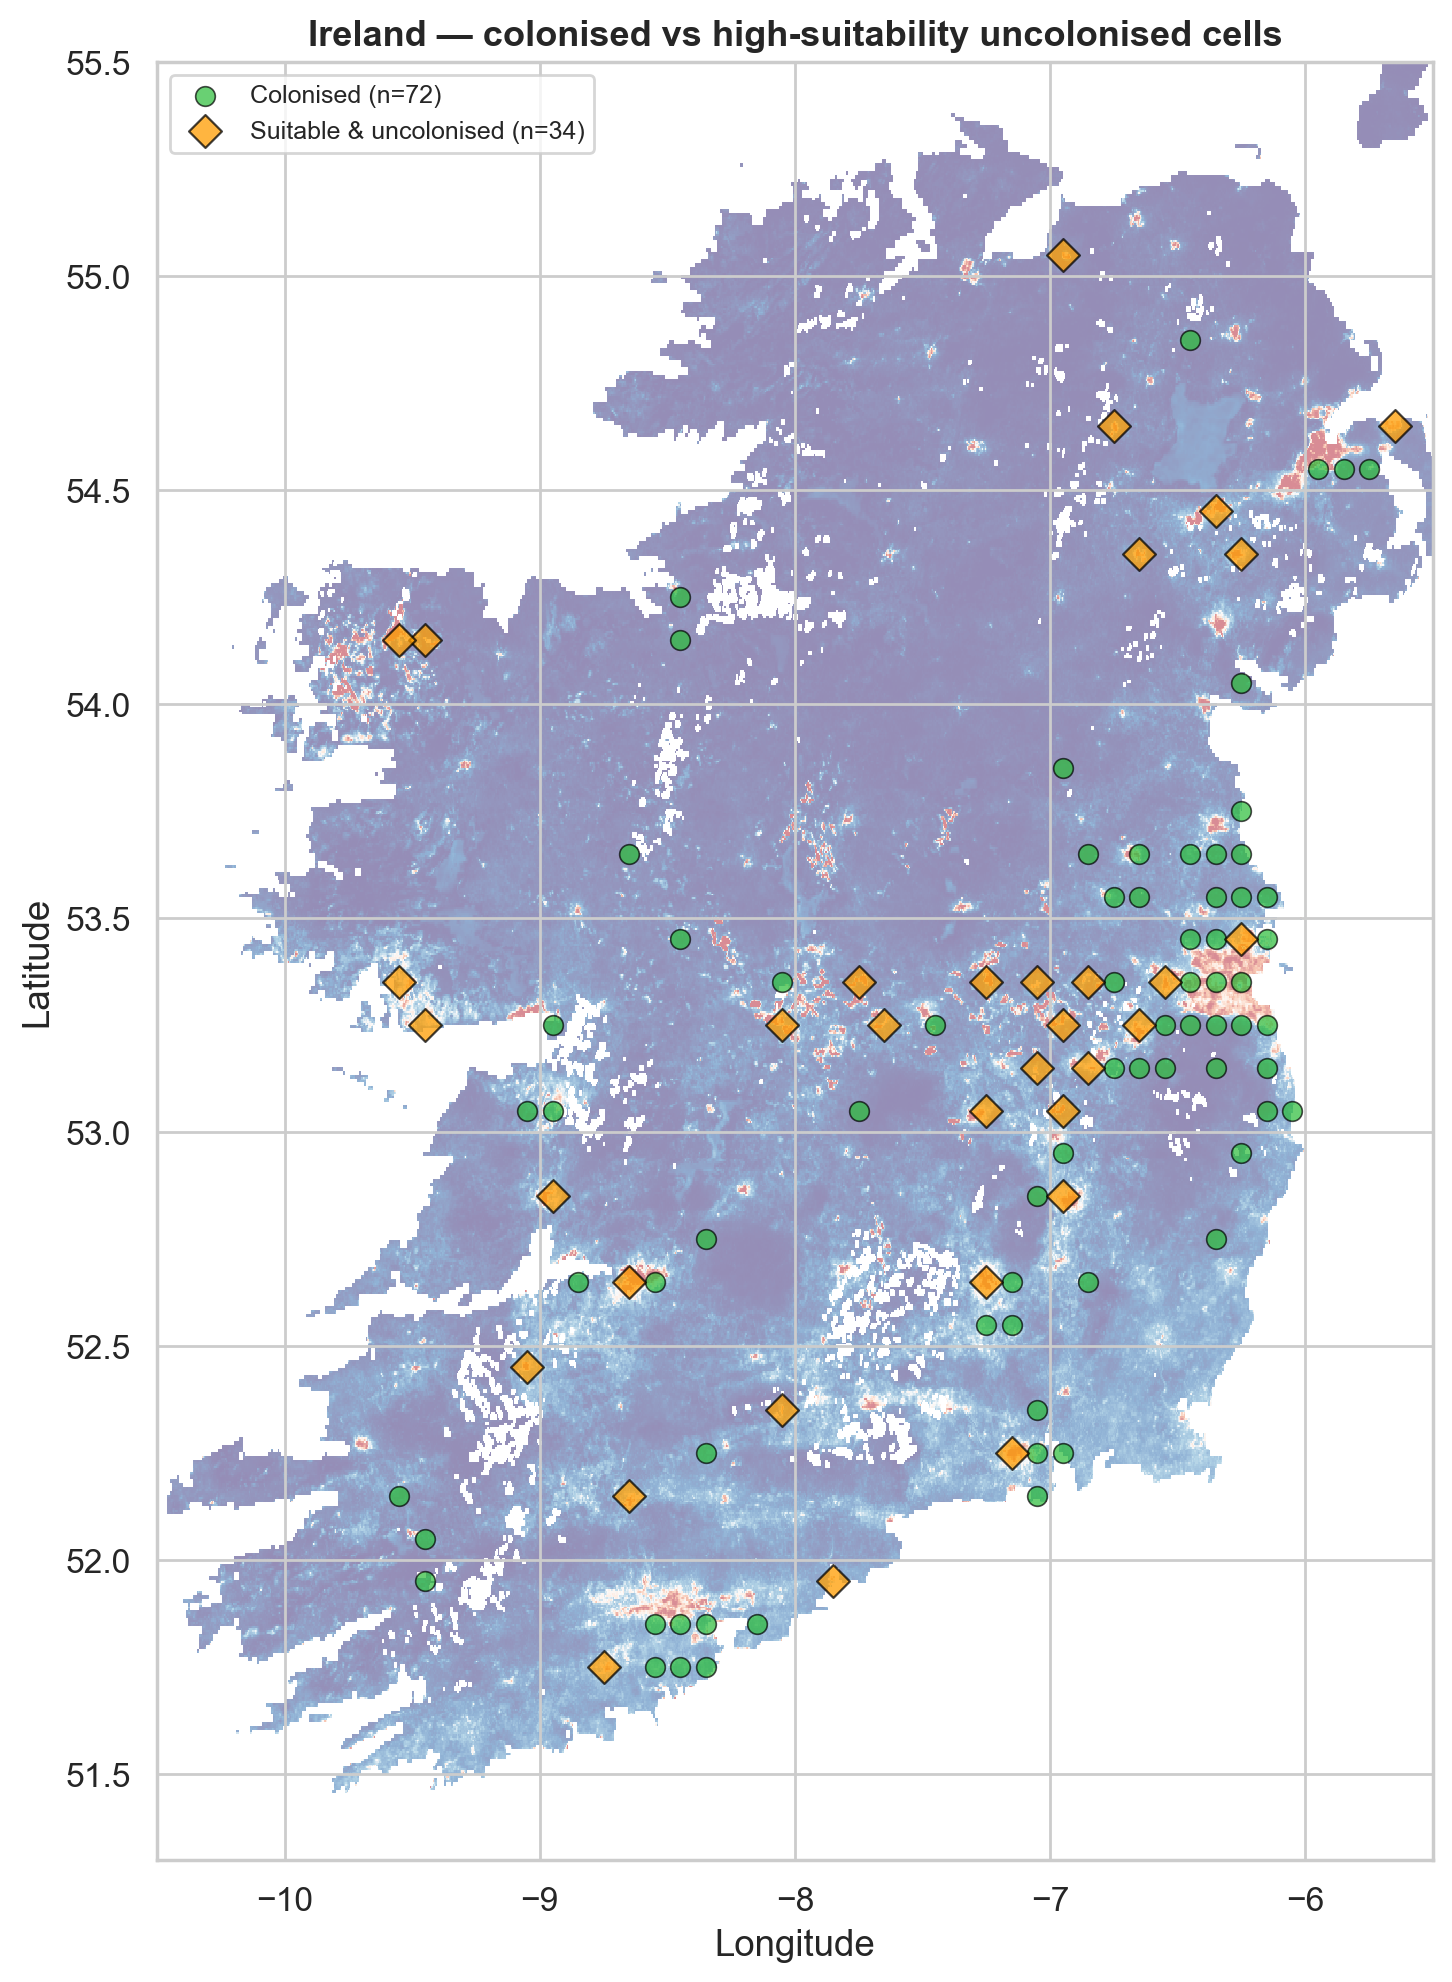
\includegraphics[width=\columnwidth]{../outputs/ireland_uncolonised_suitable.png}
\caption{Map of Ireland showing ${\sim}$10~km grid cells already colonised by \textit{S.~nobilis} (blue circles; $n = 72$) and high-suitability cells ($\geq$ 0.4) with no records to date (cyan diamonds; $n = 34$). Uncolonised suitable cells are concentrated in the midlands and regional towns such as Tullamore, Athlone, Waterford, Naas, Ennis, and Dundalk, representing the most likely sites for future establishment.}
\label{fig:uncolonised_suitable}
\end{figure}

\section{Discussion}

This study demonstrates that satellite-derived measurements of artificial light at night and land surface temperature can effectively predict the distribution of the invasive noble false widow spider \textit{S.~nobilis} across Western Europe. Using only four remotely sensed environmental variables, the MaxEnt model achieved a spatially cross-validated AUC of 0.69, correctly identifying known hotspots in southeastern England, northern France, and Irish urban centres while also highlighting areas of predicted suitability that have not yet been colonised. The temporal analysis for Ireland further showed that the species' geographic spread follows a logistic trajectory, with an estimated 90\% of suitable habitat projected to be occupied by ${\sim}$2027.

The dominance of thermal variables in the model --- MODIS daytime LST alone accounted for an AUC drop of 0.20 under permutation --- is consistent with the known physiology and ecology of \textit{S.~nobilis}. As an ectotherm of subtropical origin, the species is constrained by minimum thermal thresholds for survival and reproduction \citep{Bauer2019}. The response curve for MODIS daytime LST, which peaks at 10--14\textdegree C, corresponds closely to the mean annual temperatures of the British Isles and Atlantic France, where the species has been most successful. The decline in predicted suitability at higher daytime LST values ($>$18\textdegree C) likely reflects a modelling artefact rather than true thermal unsuitability: occurrences in the warmer Mediterranean portion of the species' native range are fewer in the citizen-science dataset, reducing the model's ability to capture suitability in those environments. Future work incorporating occurrence data from the full native range in Macaronesia and North Africa would help resolve this asymmetry.

VIIRS nighttime radiance, while ranking fourth in permutation importance, contributes ecological information that is not captured by temperature alone. Its weak correlation with the three LST variables ($r = 0.25$--$0.34$) confirms that artificial light represents an independent environmental axis. The monotonic, saturating response curve for VIIRS radiance is consistent with the hypothesis that \textit{S.~nobilis} benefits from ALAN both directly --- through increased prey availability around light sources \citep{GastonBennie2014} --- and indirectly, as a spatial proxy for the density of heated buildings and human infrastructure that provide overwintering refugia. The relatively modest contribution of ALAN to overall model performance may partly reflect the coarse spatial resolution of VIIRS (750~m native), which smooths the sharp gradients in light intensity found between individual buildings and their surroundings. Higher-resolution nighttime light data, such as those from the International Space Station or commercial satellite constellations, could potentially improve discrimination at local scales.

The spatially cross-validated AUC of 0.69 is moderate but should be interpreted in context. First, the model uses only four predictors, all derived from satellite imagery, whereas most published SDMs for terrestrial arthropods incorporate 10--20 bioclimatic and land-cover variables \citep{Elith2006}. The deliberate restriction to satellite-only predictors was a design choice intended to test the sufficiency of remotely sensed urbanisation proxies and to maximise reproducibility, as all input layers can be generated from freely available GEE archives without requiring field-collected data. Second, spatial cross-validation is known to produce substantially lower AUC values than random cross-validation when data exhibit spatial autocorrelation \citep{Roberts2017, Valavi2019}. The training AUC of 0.80 and the 0.11-point gap to the cross-validated estimate are typical of this correction. Third, the study area spans 25 degrees of latitude and encompasses considerable climatic and biogeographic heterogeneity; a model that discriminates presence from background with moderate accuracy across this entire extent is arguably more useful than one that achieves high AUC within a single country but fails to transfer.

The logistic growth analysis for Ireland provides a complementary temporal perspective on the invasion. The estimated carrying capacity of $K = 103$ grid cells ($\pm$ 23) and growth rate of $r = 0.47$~yr$^{-1}$ suggest rapid but decelerating expansion, with the inflection point already passed in ${\sim}$2022. The 34 high-suitability cells with no records to date are concentrated in the midlands and smaller regional towns --- areas where both the model and ecological reasoning suggest the species could establish, but where citizen-science recording effort is lower than in Dublin or Cork. It is important to acknowledge that some of these ``uncolonised'' cells may in fact already harbour \textit{S.~nobilis} populations that have simply not yet been reported; targeted field surveys in these areas would help distinguish true absence from recording gaps. Nevertheless, the convergence of the SDM suitability surface and the logistic saturation estimate provides a useful prioritisation framework for public health surveillance and invasive species monitoring.

Several limitations should be noted. First, the temporal window of the occurrence data (2017--2025) means that the model captures a snapshot of a species in active range expansion, and the realised niche may not yet fully represent the fundamental niche. As the species continues to spread, future records from currently unoccupied areas may shift the modelled environmental envelope. Second, the use of citizen-science data introduces biases related to recorder effort, species detectability, and identification accuracy, although the bias-corrected background sampling and restriction to research-grade records help mitigate these issues \citep{Beck2014}. Third, the model does not account for biotic interactions, dispersal barriers, or microhabitat features (e.g.\ building material, wall orientation) that likely influence local-scale occurrence but are not detectable at the 1~km resolution of the satellite data. Finally, the logistic growth model assumes a fixed carrying capacity, whereas in reality both climate change and continued urbanisation may alter the amount of suitable habitat over time.

In conclusion, freely available satellite observations of artificial light at night and land surface temperature are effective predictors of \textit{S.~nobilis} distribution at a continental scale. The species' environmental niche is defined by mild maritime daytime temperatures, moderate nocturnal warmth, warm summer surface conditions, and elevated artificial lighting --- a combination most strongly associated with urban and suburban environments in the British Isles and northern France. In Ireland, the species has colonised approximately 75\% of its predicted suitable range as of 2025, with the logistic growth model projecting near-saturation by ${\sim}$2027. The 34 high-suitability grid cells with no records to date, concentrated in the Irish midlands and regional towns, represent the most likely locations for new establishment and should be prioritised for targeted surveillance. More broadly, the approach developed here --- combining satellite-derived urbanisation proxies with citizen-science occurrence data in a presence-background SDM framework --- offers a scalable and reproducible method for monitoring synanthropic invasive species that can be readily transferred to other taxa and geographic regions. As urbanisation and artificial lighting continue to expand worldwide \citep{Kyba2017}, satellite-based monitoring of the species that track these changes will become increasingly important for biodiversity management and public health preparedness.

\section*{Acknowledgements}

We thank the thousands of citizen scientists who contributed \textit{Steatoda nobilis} observations to iNaturalist and 
GBIF, without whom this study would not have been possible. Satellite data were accessed through Google Earth Engine. 
We acknowledge the NASA MODIS, VIIRS, and Landsat science teams for producing and maintaining the remote sensing products 
used in this analysis. EPC conceived the study, developed the methodology and software, curated and analysed the data, 
produced all visualisations, and wrote the original draft. RAP contributed to the conceptualisation, supervised the work, 
and reviewed and edited the manuscript. All occurrence records are publicly available from iNaturalist 
(\url{https://www.inaturalist.org}) and GBIF (\url{https://www.gbif.org}). Satellite imagery was accessed via Google Earth 
Engine (\url{https://earthengine.google.com}). Processed data, analysis code, and model outputs are available from the 
corresponding author upon reasonable request. The authors declare no conflicts of interest.

\bibliography{references}

\end{document}
